% This is samplepaper.tex, a sample chapter demonstrating the
% LLNCS macro package for Springer Computer Science proceedings;
% Version 2.20 of 2017/10/04
%
\documentclass[runningheads]{llncs}
%
\usepackage{graphicx}
% Used for displaying a sample figure. If possible, figure files should
% be included in EPS format.
%
% If you use the hyperref package, please uncomment the following line
% to display URLs in blue roman font according to Springer's eBook style:
% \renewcommand\UrlFont{\color{blue}\rmfamily}

\begin{document}
%
\title{A review of a hybrid feature selection method for DNA microarray data}
%
%\titlerunning{Abbreviated paper title}
% If the paper title is too long for the running head, you can set
% an abbreviated paper title here
%
\author{Laura Rodríguez-Navas\orcidID{0000-0003-4929-1219}}
%
% \authorrunning{F. Author et al.}
% First names are abbreviated in the running head.
% If there are more than two authors, 'et al.' is used.
%
\institute{Universidad Internacional Menéndez Pelayo (UIMP), Madrid, Spain \\
	\email{rodrigueznavas@posgrado.uimp.es}}
%
\maketitle              % typeset the header of the contribution
%
\begin{abstract}
The emergence of DNA Microarray technology has enabled researchers to analyse the expression level of thousands of genes simultaneously. The Microarray data analysis is the process of finding the most informative genes as well as remove redundant and irrelevant genes. One of the most important applications of Microarray data analysis is cancer classification. Gene expression profiles, which represent the state of a cell at a molecular level, have great potential as a medical diagnosis tool. In cancer classification, available training data sets are generally of a small sample size compared to the number of genes involved. Along with training data limitations, this constitutes a challenge to certain classification methods. However, the curse of dimensionality and the curse of sparsity make classifying gene expression profiles a challenging task. One of the most effective methods to overcome these challenges is feature (gene) selection. The feature (gene) selection can be used to successfully extract those genes that directly influence classification accuracy, and to eliminate genes that have no influence on it. This significantly improves calculation performance and classification accuracy. In this paper, I aim to review the correlation-based feature selection (CFS), and the Taguchi-genetic algorithm (TGA) merged into a new hybrid method since the classification accuracy obtained by the proposed method is higher when it is compared to other classification methods from the literature.

\keywords{Feature selection \and Taguchi-genetic algorithm \and Leave-one-out cross-validation.}

\end{abstract}
%
%
%
\section{Introduction}

DNA Microarray technology is a powerful tool that helps researchers to monitor the gene expression level in an organism. Microarray data analysis provides valuable results which contribute towards solving gene expression profile problems. One of the most important applications of Microarray data analysis is cancer classification. Cancer may be a genetic disease; the analysis of cancer pathology in the analysis of genes that cause cancer, i.e. the gene whose mutation is responsible for cancer. This reflects the changes in the expression level of various genes. However, classifying the gene expression profile is a challenging task and considered as (NP)-Hard problem~\cite{narendra1977branch}. Hence, not all genes contribute to the presence of cancer. A vast number of genes are irrelevant or insignificant to clinical diagnosis. Therefore, incorrect diagnoses can be reached when all the genes are used in Microarray gene expression classification. There are two main issues related to the analysis of Microarray data; first, the dataset in Microarray is high-dimensional which means it contains several thousand genes (features) and it has low data sparsity, meaning it has a low number of samples, usually tens of samples. Second, gene expression data has a high complexity; genes are directly or indirectly correlated to each other. Standard machine learning methods did not perform well because these methods are best suited when there are more samples than features.

To overcome these issues, dimension reduction or feature (gene) selection algorithms have been applied. Generally, gene selection methods are categorized into three categories: filter, wrapper and embedded methods. The filter approach separates data before the actual classification process takes place and then calculates feature weight values, and thus features that accurately present the original data set can be identified. However, a filter approach does not account for interactions amongst the features. The method in the filter approach category is described in section~\ref{Correlation-based feature selection}. Wrapper models, on the other hand, generally are focused on improving classification accuracy of pattern classification problems and typically perform better (i.e., reach higher classification accuracy) than filter models. However, wrapper approaches are more computationally expensive than filter methods. Several methods in this category have previously been used to perform feature selection of training and testing data, such as genetic algorithm (GA) which is described in section~\ref{Genetic algorithm}. And the embedded techniques use an inductive algorithm. The inductive algorithm itself represents the feature selector and the classifier, searching for an optimal subset of features that are built into the classifier. The advantage of embedded algorithms is that they take the interaction with the classifier into account. A disadvantage of embedded algorithms is that they are generally based on a greedy mechanism, i.e., they only use top-ranked attributes to perform sample classification~\cite{saeys2007review}\cite{yang2010multi}.

Recently, hybrid and ensemble methods were added to the general framework of feature selection. A hybrid approach is built to take advantage of both filter and wrapper approaches. Thus, it combines the computational efficiency of the filter approach with the high performance of the wrapper approach. A hybrid feature selection approach consisting of two stages is presented in this review. The first stage involves a filter approach that is used to calculate correlation-based feature weights for each feature, thus identifying relevant features. And the second stage constitutes a wrapper approach, i.e. the previously identified relevant feature subsets are tested by a Taguchi-genetic algorithm (TGA), which tries to determine optimal feature subsets. The optimal performance of the hybrid approach is dependent on two factors; the classification accuracy and the number of selected genes.

\section{Feature (gene) selection methods}

\subsection{Correlation-based feature selection}\label{Correlation-based feature selection}
Correlation-based feature selection (CFS) was developed by Hall in 1999~\cite{hall1998correlation}.

\subsection{Genetic algorithm}\label{Genetic algorithm}

\subsection{Taguchi method}

\section{CFS–TGA method}

\section{Conclusions}

\begin{equation}
x + y = z
\end{equation}
Please try to avoid rasterized images for line-art diagrams and
schemas. Whenever possible, use vector graphics instead (see
Fig.~\ref{fig1}).

\begin{figure}
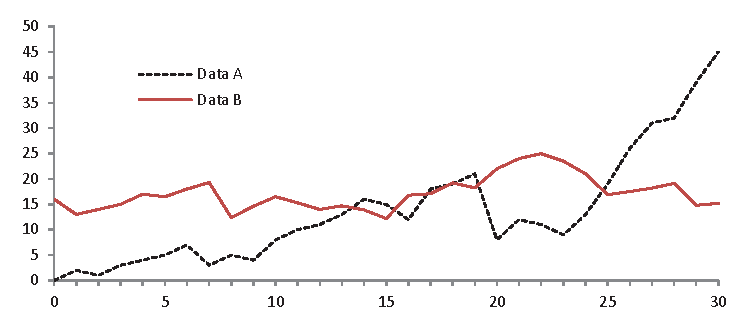
\includegraphics[width=\textwidth]{fig1.eps}
\caption{A figure caption is always placed below the illustration.
Please note that short captions are centered, while long ones are
justified by the macro package automatically.} \label{fig1}
\end{figure}
%
% ---- Bibliography ----
%
% BibTeX users should specify bibliography style 'splncs04'.
% References will then be sorted and formatted in the correct style.
%
\nocite{*}

\bibliographystyle{splncs04}
\bibliography{samplepaper}
%
\end{document}
